\documentclass[11pt]{article}

% Insert style guide
\usepackage{my_thesis}
% Specifiy the location of images to be used
\graphicspath{{figures/}}

\begin{document}
\title{\textsc{Plasma based Structured Illumination Microscopy}\\}
\date{\footnote{Last Modified: \currenttime, \today.}}
\maketitle


\section{Abstract}
%
A high-reso
We present a linear high-resolution imaging scheme based on the plasma waves originating in the channel of field-effect transistors. The extremely small plasmonic wavelength along with a tunable illumination pattern in the far infrared region can resolve nano-scale objects over a broad range of frequencies.
%
\section{Introduction}
%
Conventional wide-field fluorescent microscopy employs uniform lateral illumination of the sample to observe in the farfield through the objective lens. The uniform nature of the light source fundamentally restricts the resolution of the system to half the light source wavelength due to Abbe diffraction limit. In order to meet ever increasing need to obtain high resolution particularly in life sciences, modern microscopy techniques such as confocal and linear structured illumination microscopy use spatially non-uniform sources to illuminate the sample, resulting in achieving resolution beyond the diffraction limit by a factor of $2$ \cite{Minsky_1988,Gustafsson_2005}. In confocal microscopy, a focused beam generated through a pinhole illuminates a portion of the sample. which is raster scanned by laterally shifting the beam to generate an image of the whole sample. On the detector side of the microscope, the image passes through another pinhole. Although the use of pinholes increases the resolution, confocal microscopy is a slow imaging technique. Moreover, part of light is discarded by the pinhole which may leave the signal strength from weakly fluorescent samples undetectably low. Structured Illumination microscopy (SIM) is a wide-field technique in which a fine illumination pattern such as a sinusoidal standing wave is used to generate \emph{Moiré fringes} in the observed image. The high frequency content is mathematically reconstructed from a series of images acquired by shifting the pattern, yielding a high resolution image.

The idea of illuminating the sample with surface waves having wavelength much smaller than free-space wavelength at the same frequency was first proposed in \cite{Nassenstein_1970} resulting in super-resolution. Surface plasmons existing at a metal-dielectric interface were used to excite a sample at optical frequencies in \cite{Wei_2010}. Similarly, in the mid-infrared frequency region, using graphene plasmons was proposed to achieve resolution two orders of magnitude beyond  the diffraction limit \cite{Zeng_2014}.

Two-dimensional electron gas (2DEG) is a tightly confined sheet of free electrons formed at the interface of semiconductor hetero-junctions in transistor-like structures. By virtue of the high electron concentration and unusually high mobility, the 2DEG exhibits extraordinary electromagnetic properties and physical phenomena \cite{Andress_2012,Tsui_1982,Reyren_2007}.
Plasma waves originating in the two-dimensional electron channel of field-effect transistors, discovered more than 30 years ago have lately received interest because of the potential to realize terahertz frequency sources and sensors \cite{Dyakonov_1993,Dyakonov_1996,Popov_2008,Otsuji_2006,Muravjov_2010}. For micron order lengths, the channel becomes a plasma cavity where the resonant frequency lies in the far-infrared (terahertz) frequency region and remarkably, can be tuned by varying the gate voltage. The gate bias also controls the electron velocity in the channel ranging from $.1 - 10 \times 10^6 m/s$ \cite{Burke_2000}. The 2DEG mobility below liquid nitrogen temperature (77 K) is very high $\approx 10^4 cm^2 V^{−1} s^{−1}$ \cite{Muravjov_2010}, resulting in undamped and low loss oscillations in the channel. It must be mentioned that substantial loss is introduced at room temperature because the mobility drops by at least two orders than the one listed above.

In this paper, we propose an extended structured illumination microscopy using plasma waves as the illumination source. The resolution enhancement is proportional to the wavenumber, which in our case can reach up to 100.

\section{Generating Illumination pattern}

% High mobility is one of the most significant properties of a 2DEG that leads to ballistic transport of electrons in the channel with minimum scattering. To solve for the dispersion relation,

We consider a Gallium Nitride / Aluminum Gallium Arsenide (GaN/AlGaN) heterostructure with material properties derived from \cite{Muravjov_2010} as shown in Fig. \ref{fig:scheme}. The GaN substrate is highly doped from the bottom to construct the gate terminal while the thicknes $d$ of AlGaN barrier layer is $20 \mathrm{nm}$. The 2DEG region can be described in terms of a surface conductivity given by:
\begin{equation}
  \sigma_s(\O) = \frac{N_s e^2 \tau_{p}}{m^{\ast}}\frac{1}{1 + j \O \tau}
  \label{eq:conductivity}
\end{equation}
%
where $N_s$ is surface charge density, $e$ is electron charge, $m^{\ast}$ is the effective mass of the 2D electrons and $\tau$ is the electron scattering time in the channel related to mobility $\u$ by $\tau = \u m^{\ast}/e$. The material properties are listed in \ref{tab:data}. Ignoring scattering effects and assuming the 2DEG is located between two dielectric halfspaces, the dispersion relation for a $\mathrm{TM}_x$ excited plane wave is expressed as \cite{Nakayama_1974}:
%
\begin{equation}
  \frac{\E_1}{k_{z1}} + \frac{\E_2}{k_{z2}} = -\frac{\sigma_s(\O)}{\O}
  \label{eq:disp_TM_two}
\end{equation}
%
where $\E_1$ and $\E_2$ are the dielectric constants of the barrier and substrate layers respectively and $k_{zi} = \sqrt{k_0^2 \E_i(\O) -  k_x^2}$ is the transverse propagation constant with $k_0$ being the free-space propagation constant. In the non-retarded regime($k_x >> k_0$), the solution for the lateral wavenumber $k_x$ from \eqref{eq:disp_TM_two} can be approximated as \cite{Jablan_2009}:
%
\begin{equation}
  k_x \approx \O \frac{\E_1 + \E_2}{\sigma_s(\O)}
  \label{eq:disl_sol}
\end{equation}
%
% Compared to $k_0$, it is noted that $k_x$



\section{Imaging Technique}
%
The SIM technique can be split into two operations; one at the sample end and the other on the microscope end. First, the sample is illuminated with a non-uniform, modulated pattern of sinusoidal shape. Only the portion of the sample that falls under the peak of the illumination signal is focused while the rest of the sample remains unfocused. Other portions are focused by laterally shifting the illumination pattern.
1. It creates optical sectioning that is excite different lateral portions of the sample by shifting of the pattern. The portion of the sample that is illuminated by the peak of the pattern is excited and it fluoresces while the rest of the sample is illuminated homogeneously by a uniform pattern. When the pattern is shifted, other portions of the sample are illuminated. This way the whole sample can be sequentially illuminated with high localized focused areas.

2. The other part of SIM deals with generation of Moiré effect that actually results in high resolution. The effect is created when the illumination signal is modulated by the sample signal
The objective lens of a microscope can be considered as a low-pass filter due to diffraction. The impulse response of the filter, i.e., the image of a point source, is a blurred spot termed as the \emph{point spread function}(PSF) of the microscope. When a sample that can be represented by $f(x,y)$ is illuminated by a signal $i(x,y)$, the output image, $m(x,y)$ of the microscope can be written in the spatial domain as \cite{Jost_2013}:
In terms of filter theory, the objective lens of a microscope can be considered as a diffraction limited low-pass filter that has a passband spanning up to $2k_0$ under ideal circumstances where $k_0$ is the free-space wavenumber. The impulse response of the filter, i.e., the image of a point source, is a blurred spot termed as the \emph{point spread function}(PSF) of the microscope. When a sample that can be represented by $f(x,y)$ is illuminated by a signal $i(x,y)$, the output image, $m(x,y)$ of the microscope can be written in the spatial domain as \cite{Jost_2013}:
%
The SIM technique requires acquisition of at least three images of the sample by laterally shifting the illumination pattern in order to correctly reconstruct the sample. In this scheme, the pattern can be laterally shifted by varying the components of a TM polarized beam exciting the structure expressed as, $\v E_{ext} = a \v{\^x} + b \v{\^z}$ so that the total field intensity becomes:
\begin{equation}
  \begin{split}
    \vert E \vert^2 &= (a + \cos k_xx)^2 + (b + \sin k_xx)^2 \\
    &=  a^2 + b^2 + 1 + 2 \chi \cos(k_xx + \psi)
  \end{split}
  \label{eq:shift}
\end{equation}
%
where $\chi = \sqrt{a^2 + b^2}$ and $\psi = \atan (b/a)$. An example of phased shift is shown in \figure

\begin{table}[h]
  \renewcommand{\arraystretch}{1.3}
  \caption{Material properties of $\mathrm{GaN/AlGaN}$ heterostructure \cite{Muravjov_2010}}
  \label{table_example}
  \centering
  \begin{tabular}{c||c}
    \hline
    $N_s$ & $7.5 10^{12} cm^{-2}$\\ \hline
    $\E_{1}$ & $9.5$ \\  \hline
    $\E_2$ & $9.6$ \\  \hline
    $d$ & $20 \mathrm{nm}$ \\  \hline
    $L$ &  $2 \mathrm{nm}$ \\  \hline
    $m^{\ast}$ & $.2 m_e$ \\  \hline
    $\tau_{77 K}$ & $1.14 \times 10^{-12} \mathrm{s} $ \\  \hline
    $\u_{77 K}$ & $10^4  \mathrm{cm^2 V^{-1} s^{-1}} $ \\  \hline
    $\tau_{295 K}$ & $.14 \times 10^{-12} \mathrm{s} $ \\  \hline
    $\u_{295 K}$ & $1200  \mathrm{cm^2 V^{-1} s^{-1}} $ \\  \hline
  \end{tabular}
  \label{tab:data}
\end{table}

\begin{figure}[h!]
  \centering
  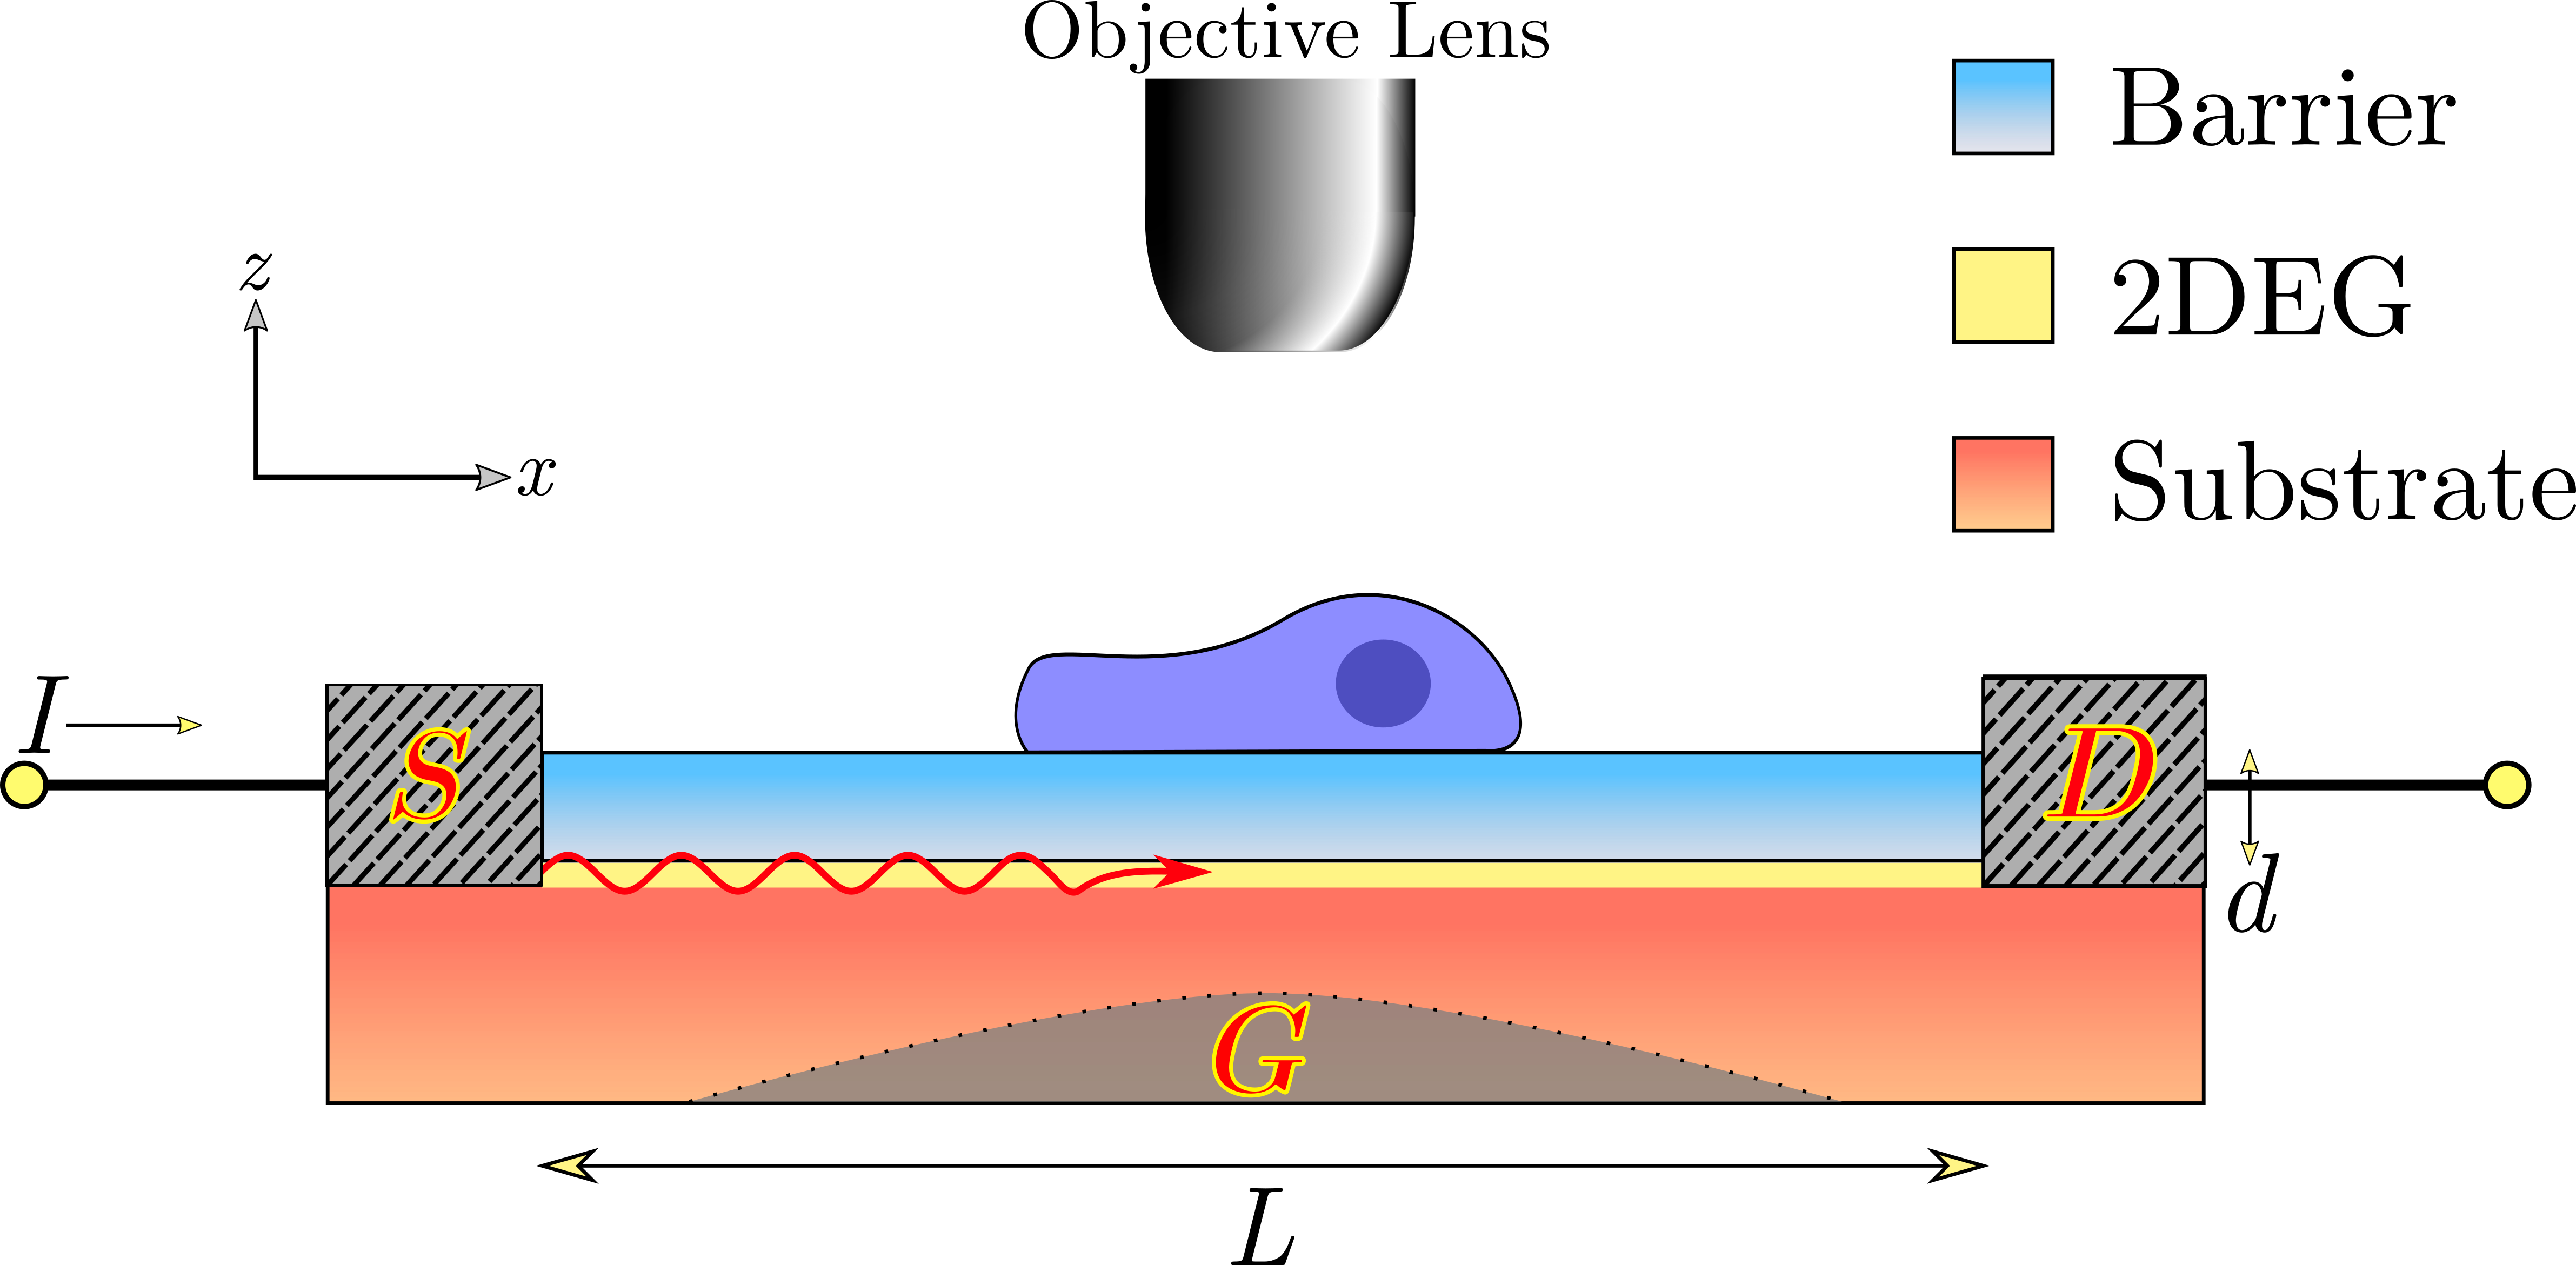
\includegraphics[scale=.5]{Microcopic_Structure.png}
  \caption{Schematic of the structure. 2DEG exists between a barrier layer of thickness $d$ and substrate}
  \label{fig:scheme}
\end{figure}

\begin{figure}[h!]
  \centering
  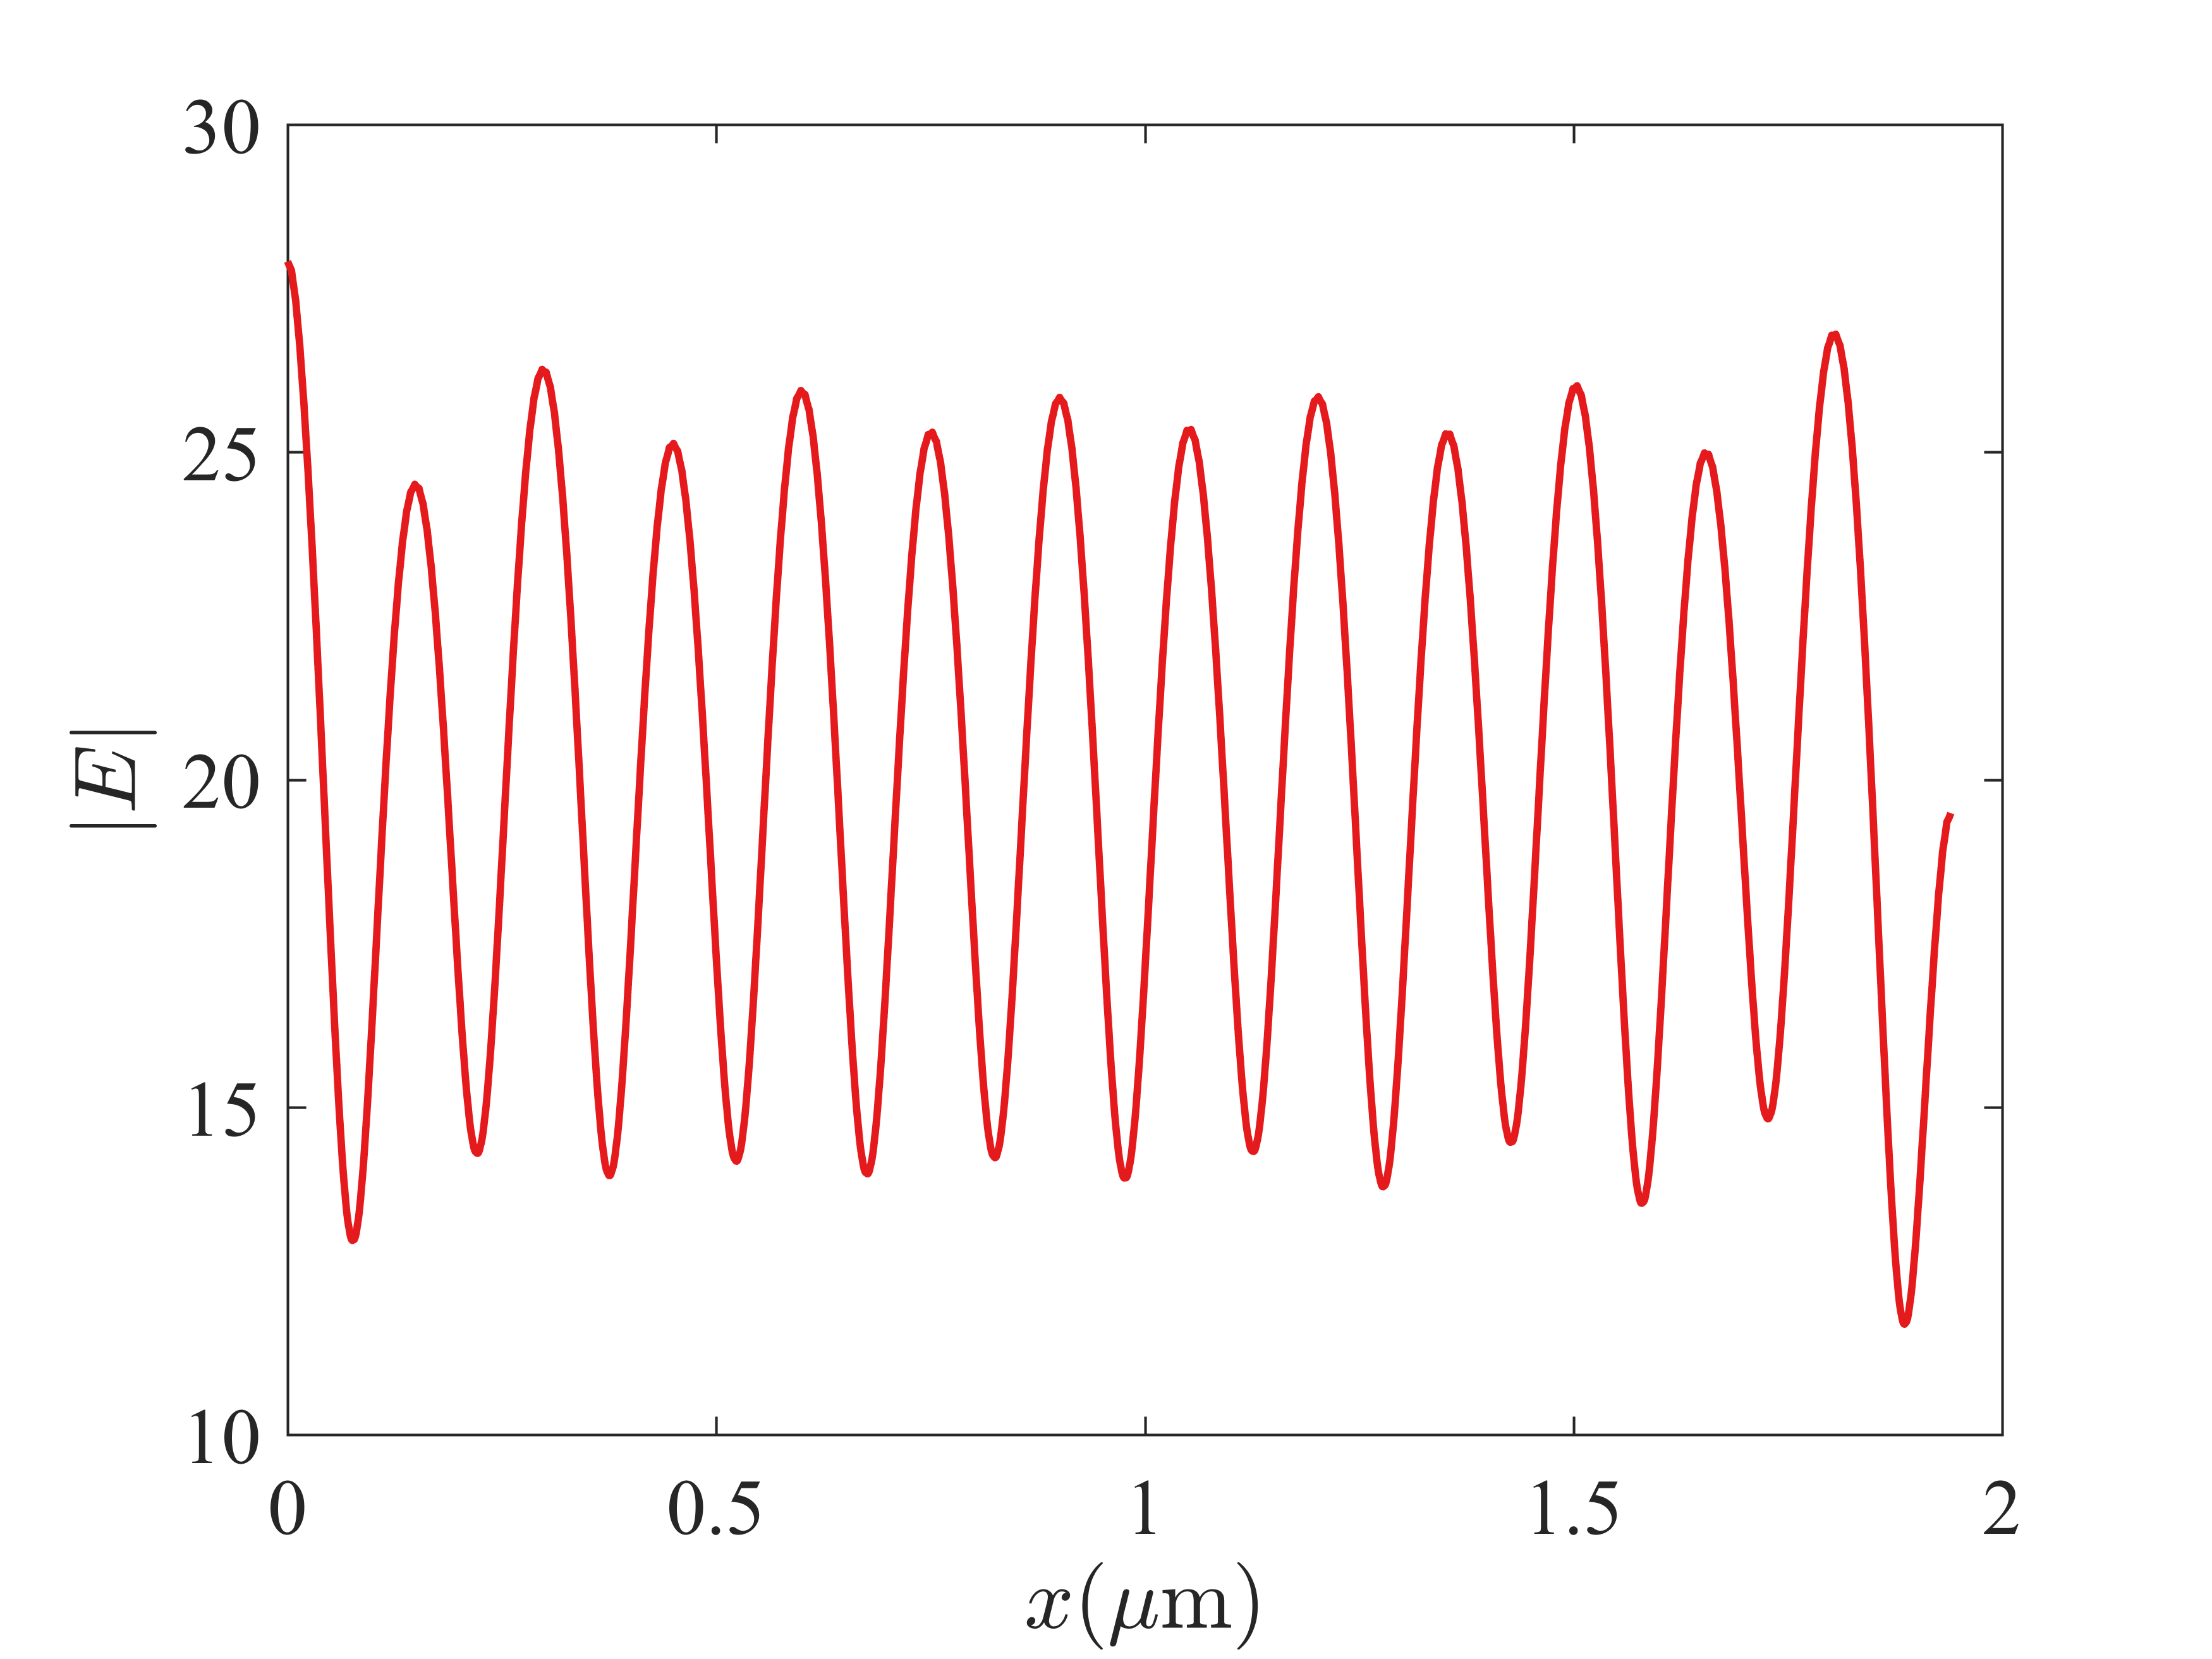
\includegraphics[scale=.5]{no_port.png}
  \caption{Absolute value of electric field along the $2 \u \mathrm{m} $ long channel GaAs/AlGaAs heterostructure}
  \label{fig:standing_wave}
\end{figure}

\begin{figure}[h!]
  \centering
  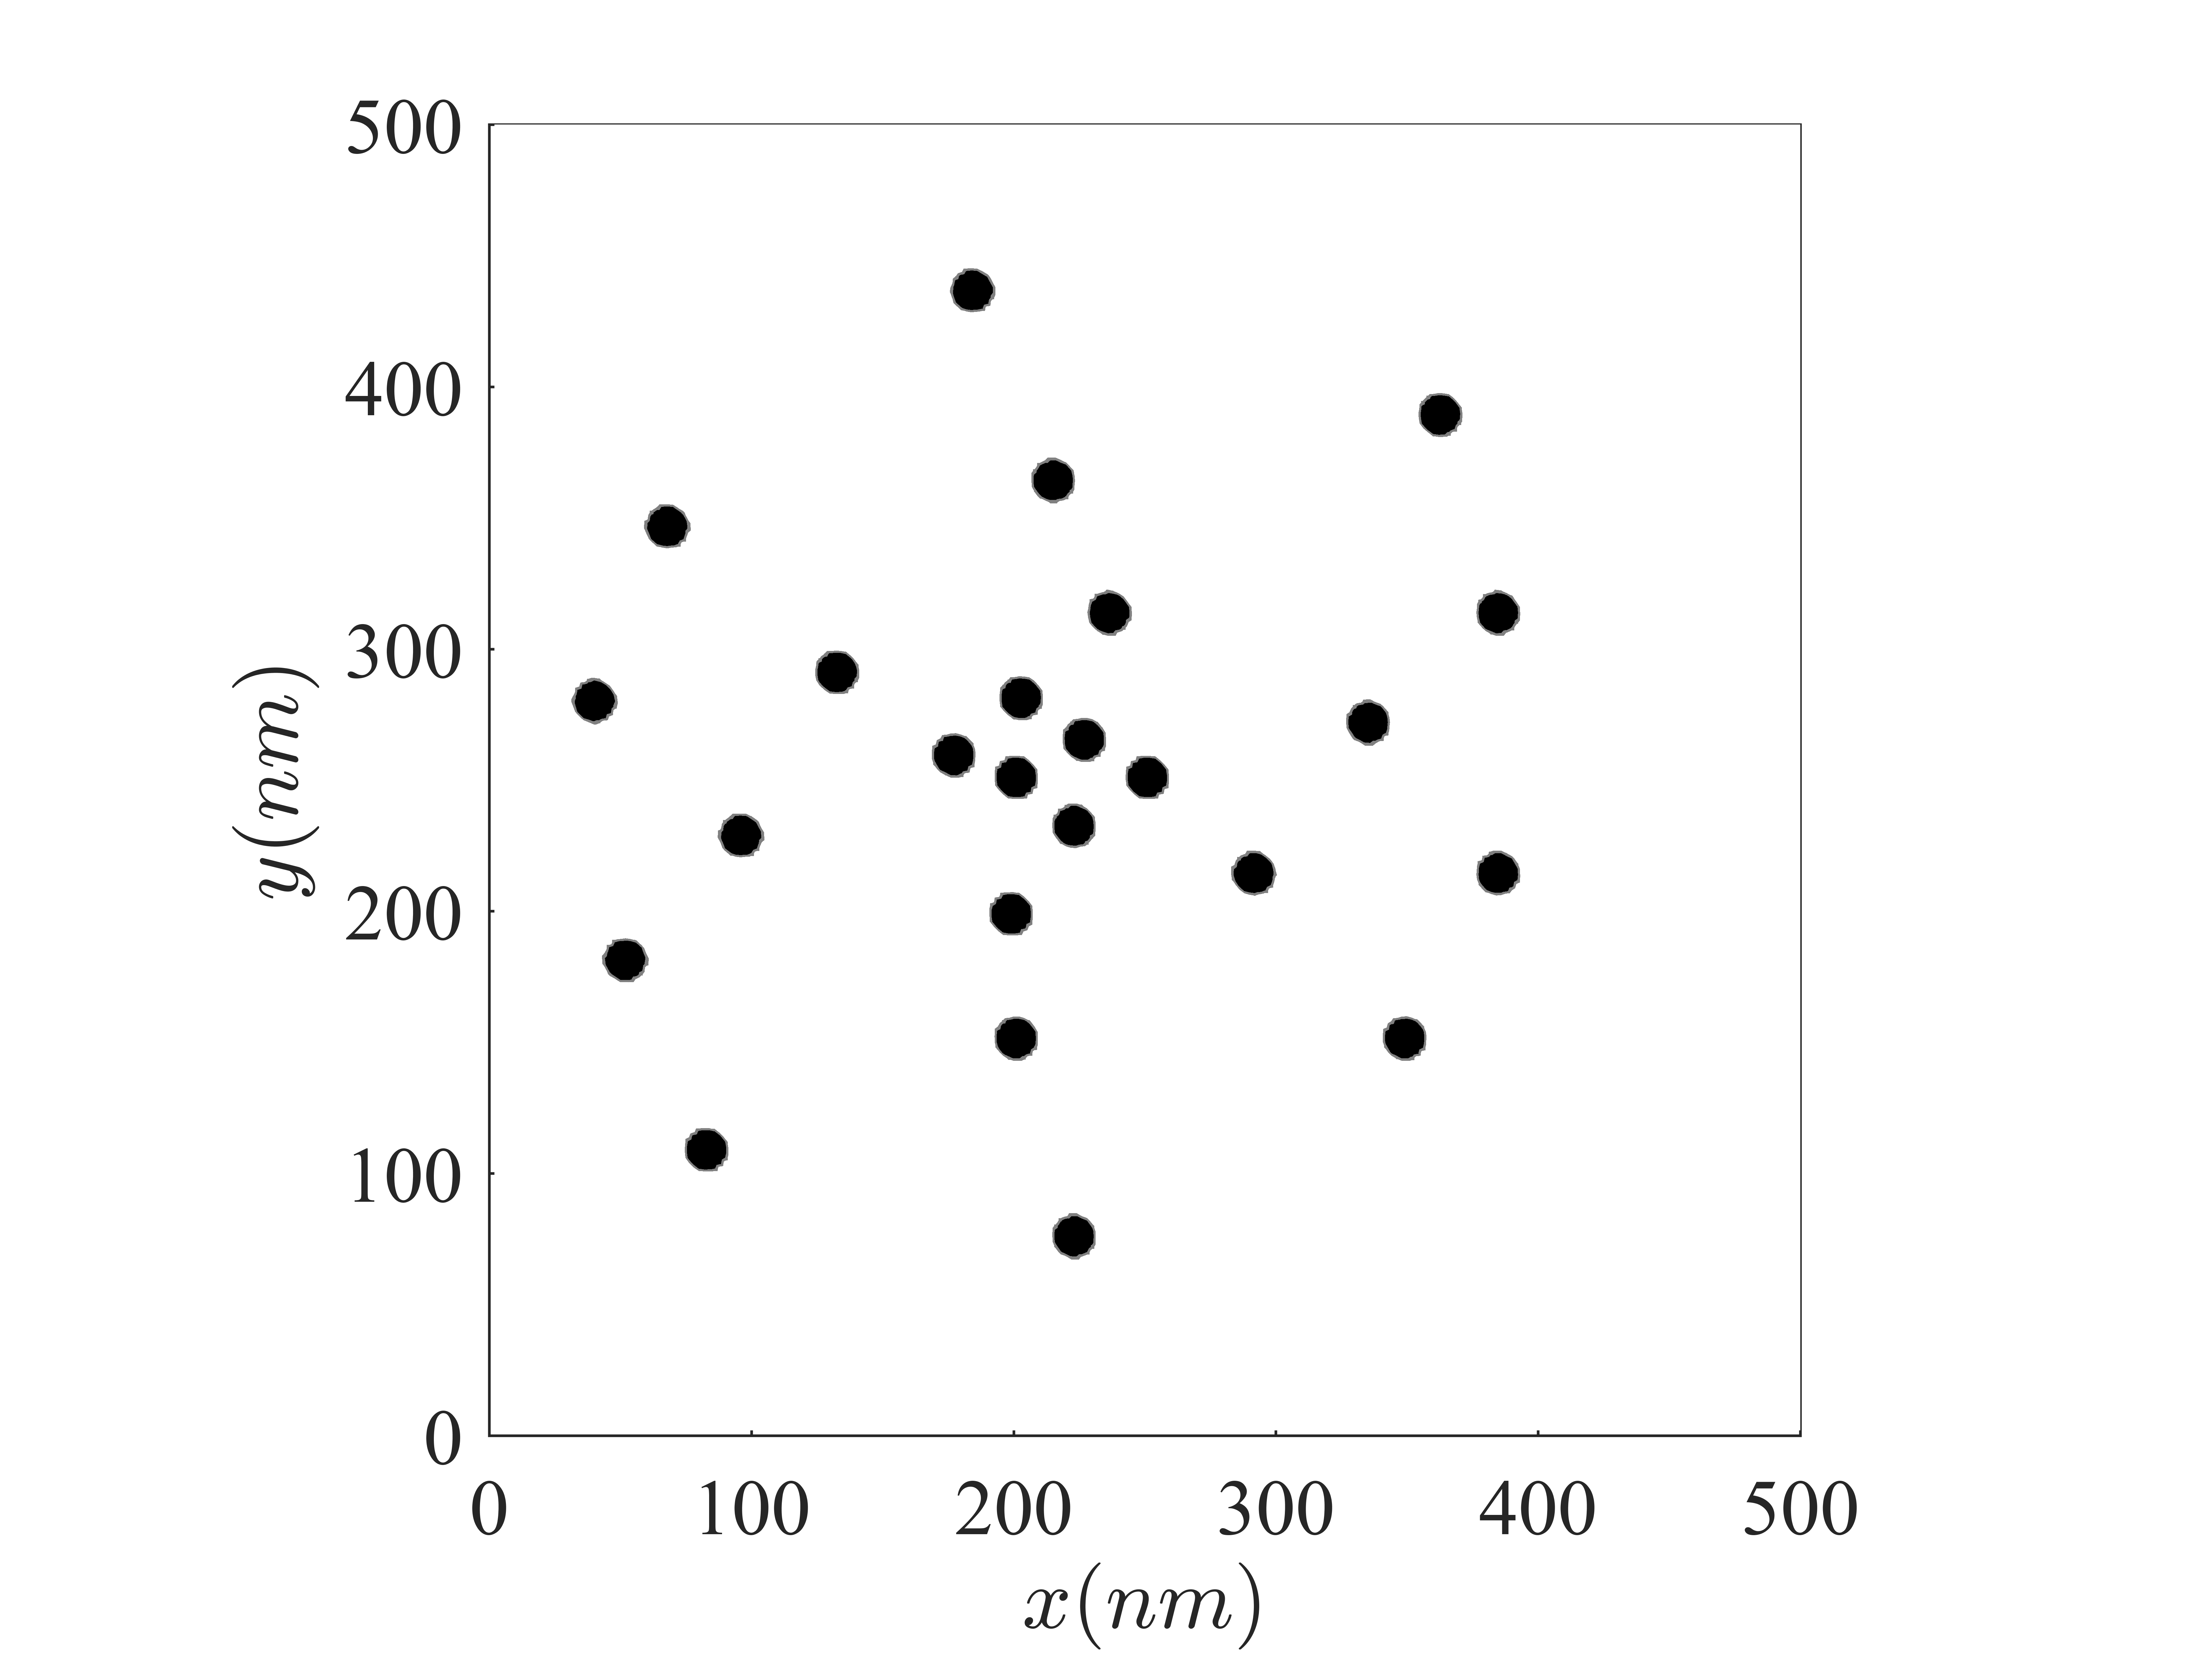
\includegraphics[scale=1]{test.png}
  \caption{Test image with $15$ nm fluorescent beads in a $500$ nm square space}
  \label{fig:scheme}
\end{figure}

\begin{figure}[h!]
  \centering
  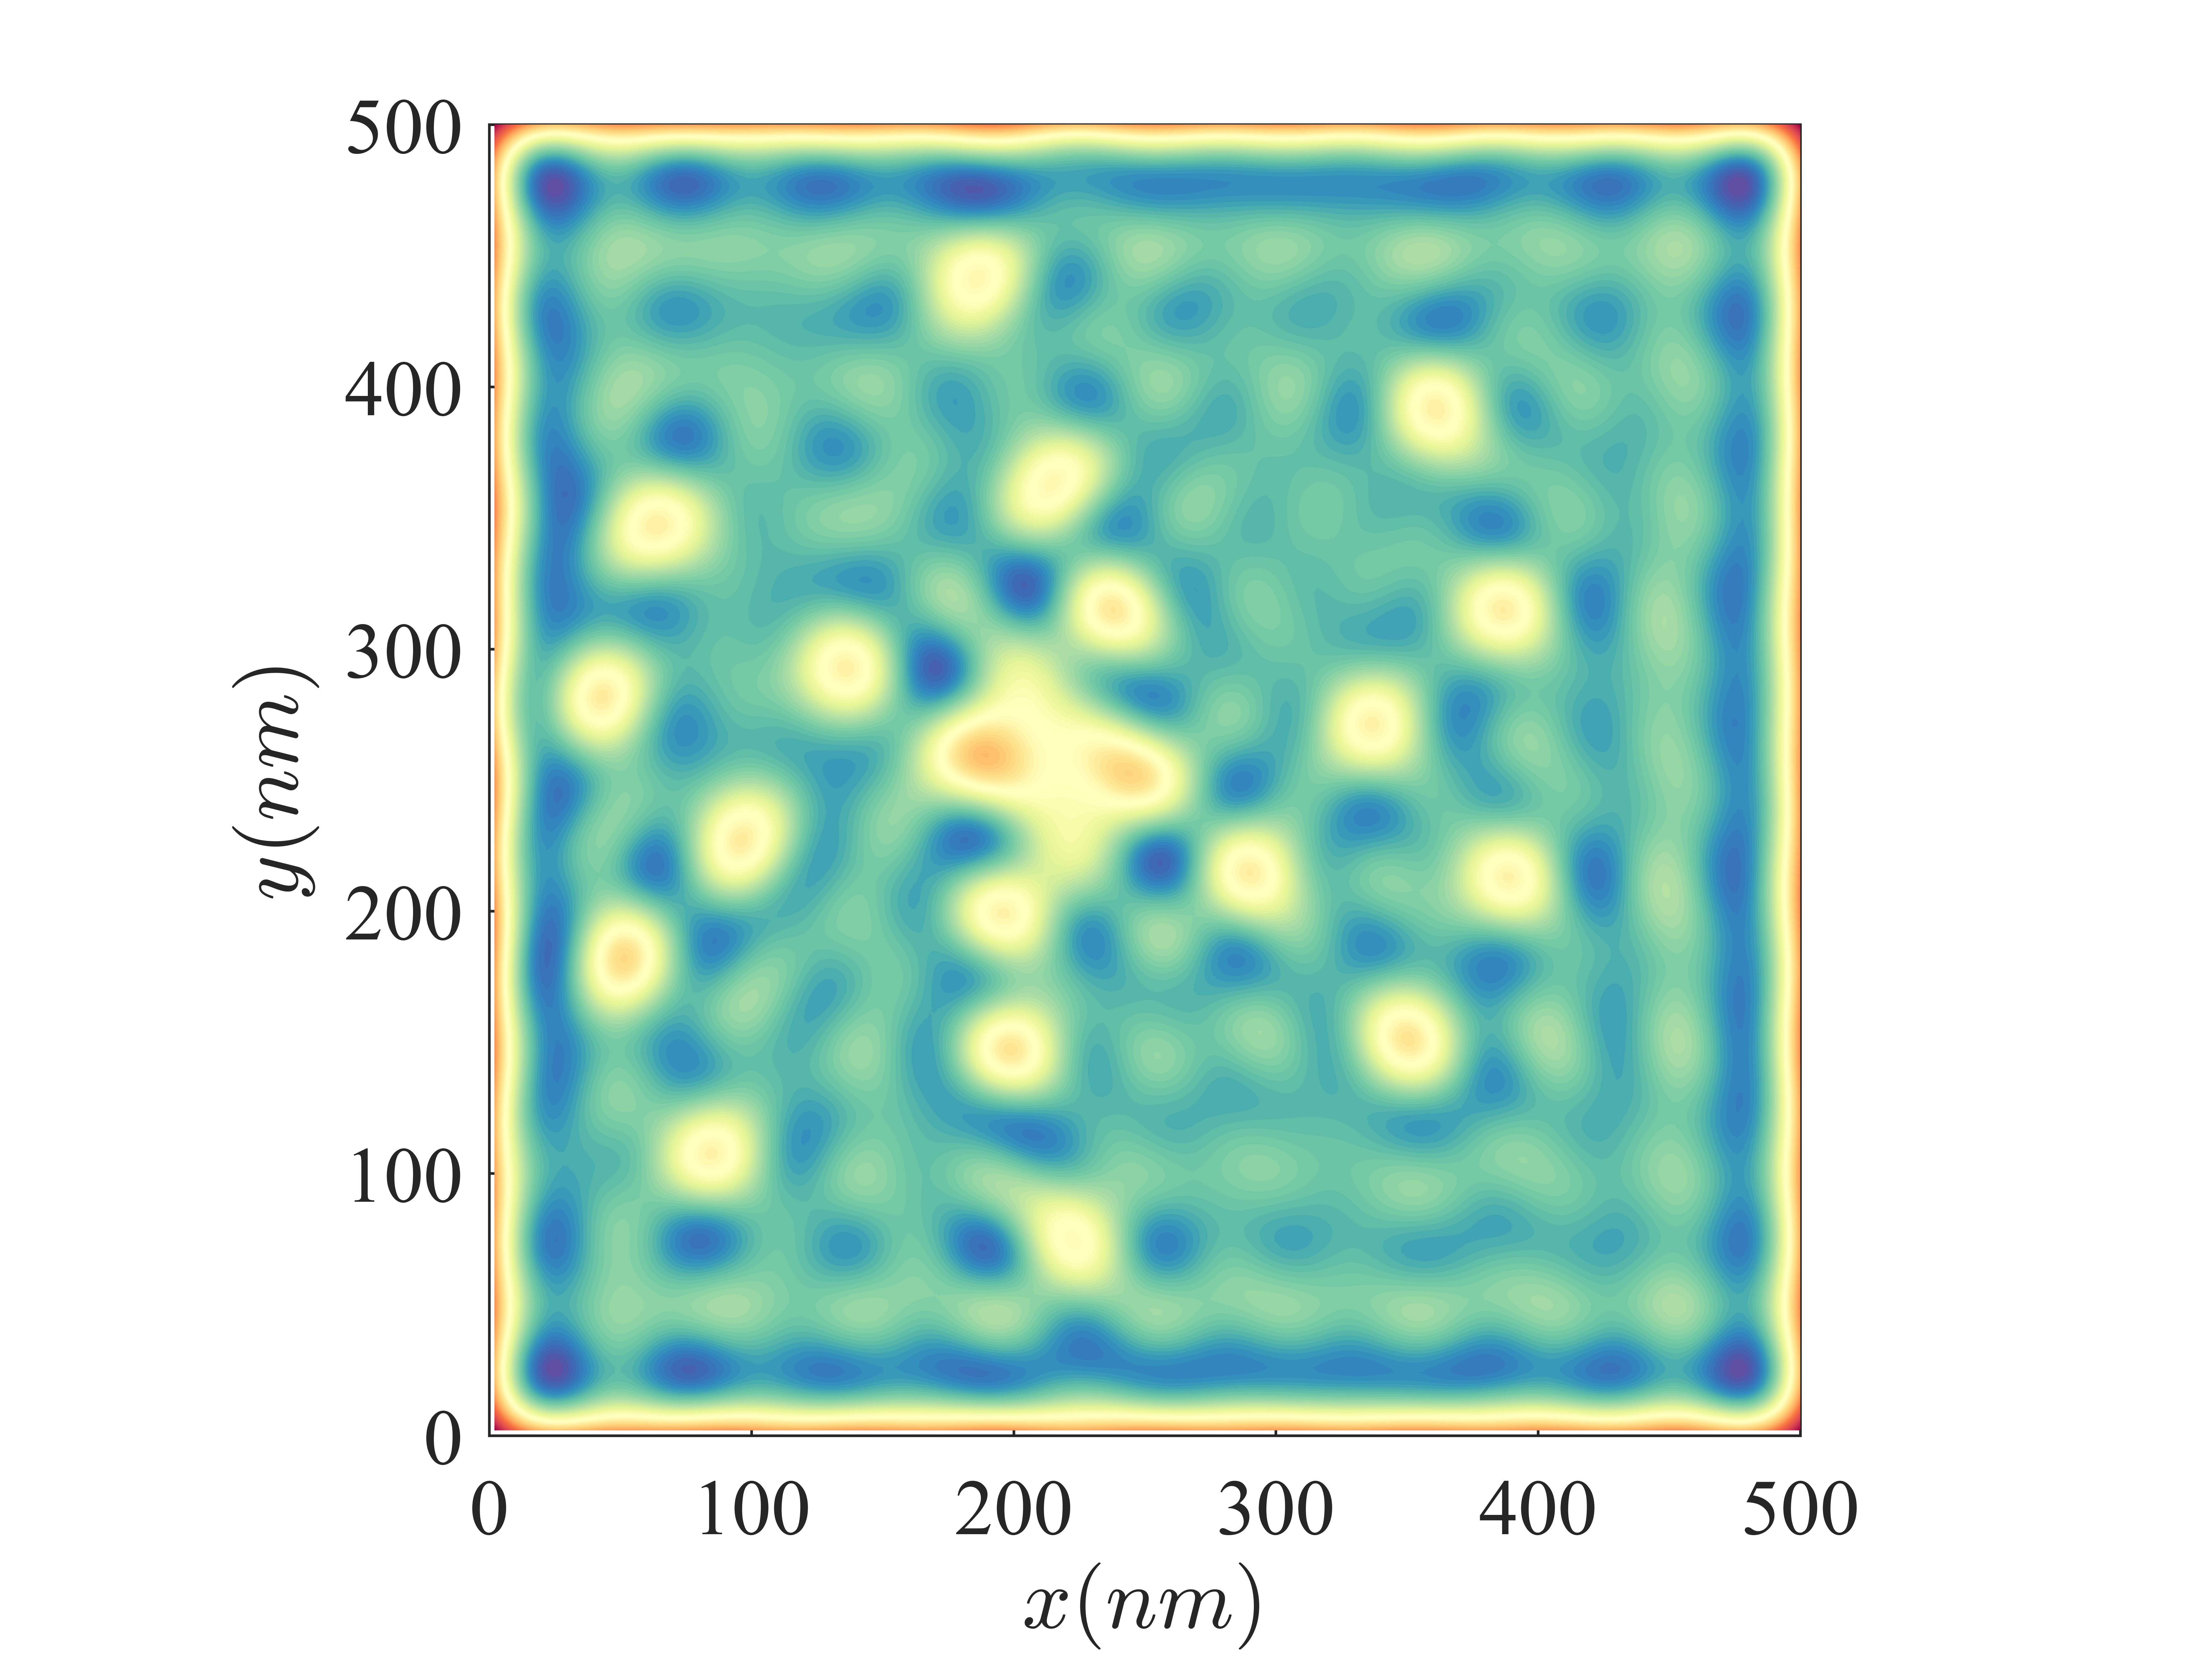
\includegraphics[scale=1]{free_space_sim.png}
  \caption{Simulation with GaN/AlGaN 2DEG at $20$ THz corresponding to $\Re(k_p) = 39 k_0$}
  \label{fig:sim_low}
\end{figure}

\begin{figure}[h!]
  \centering
  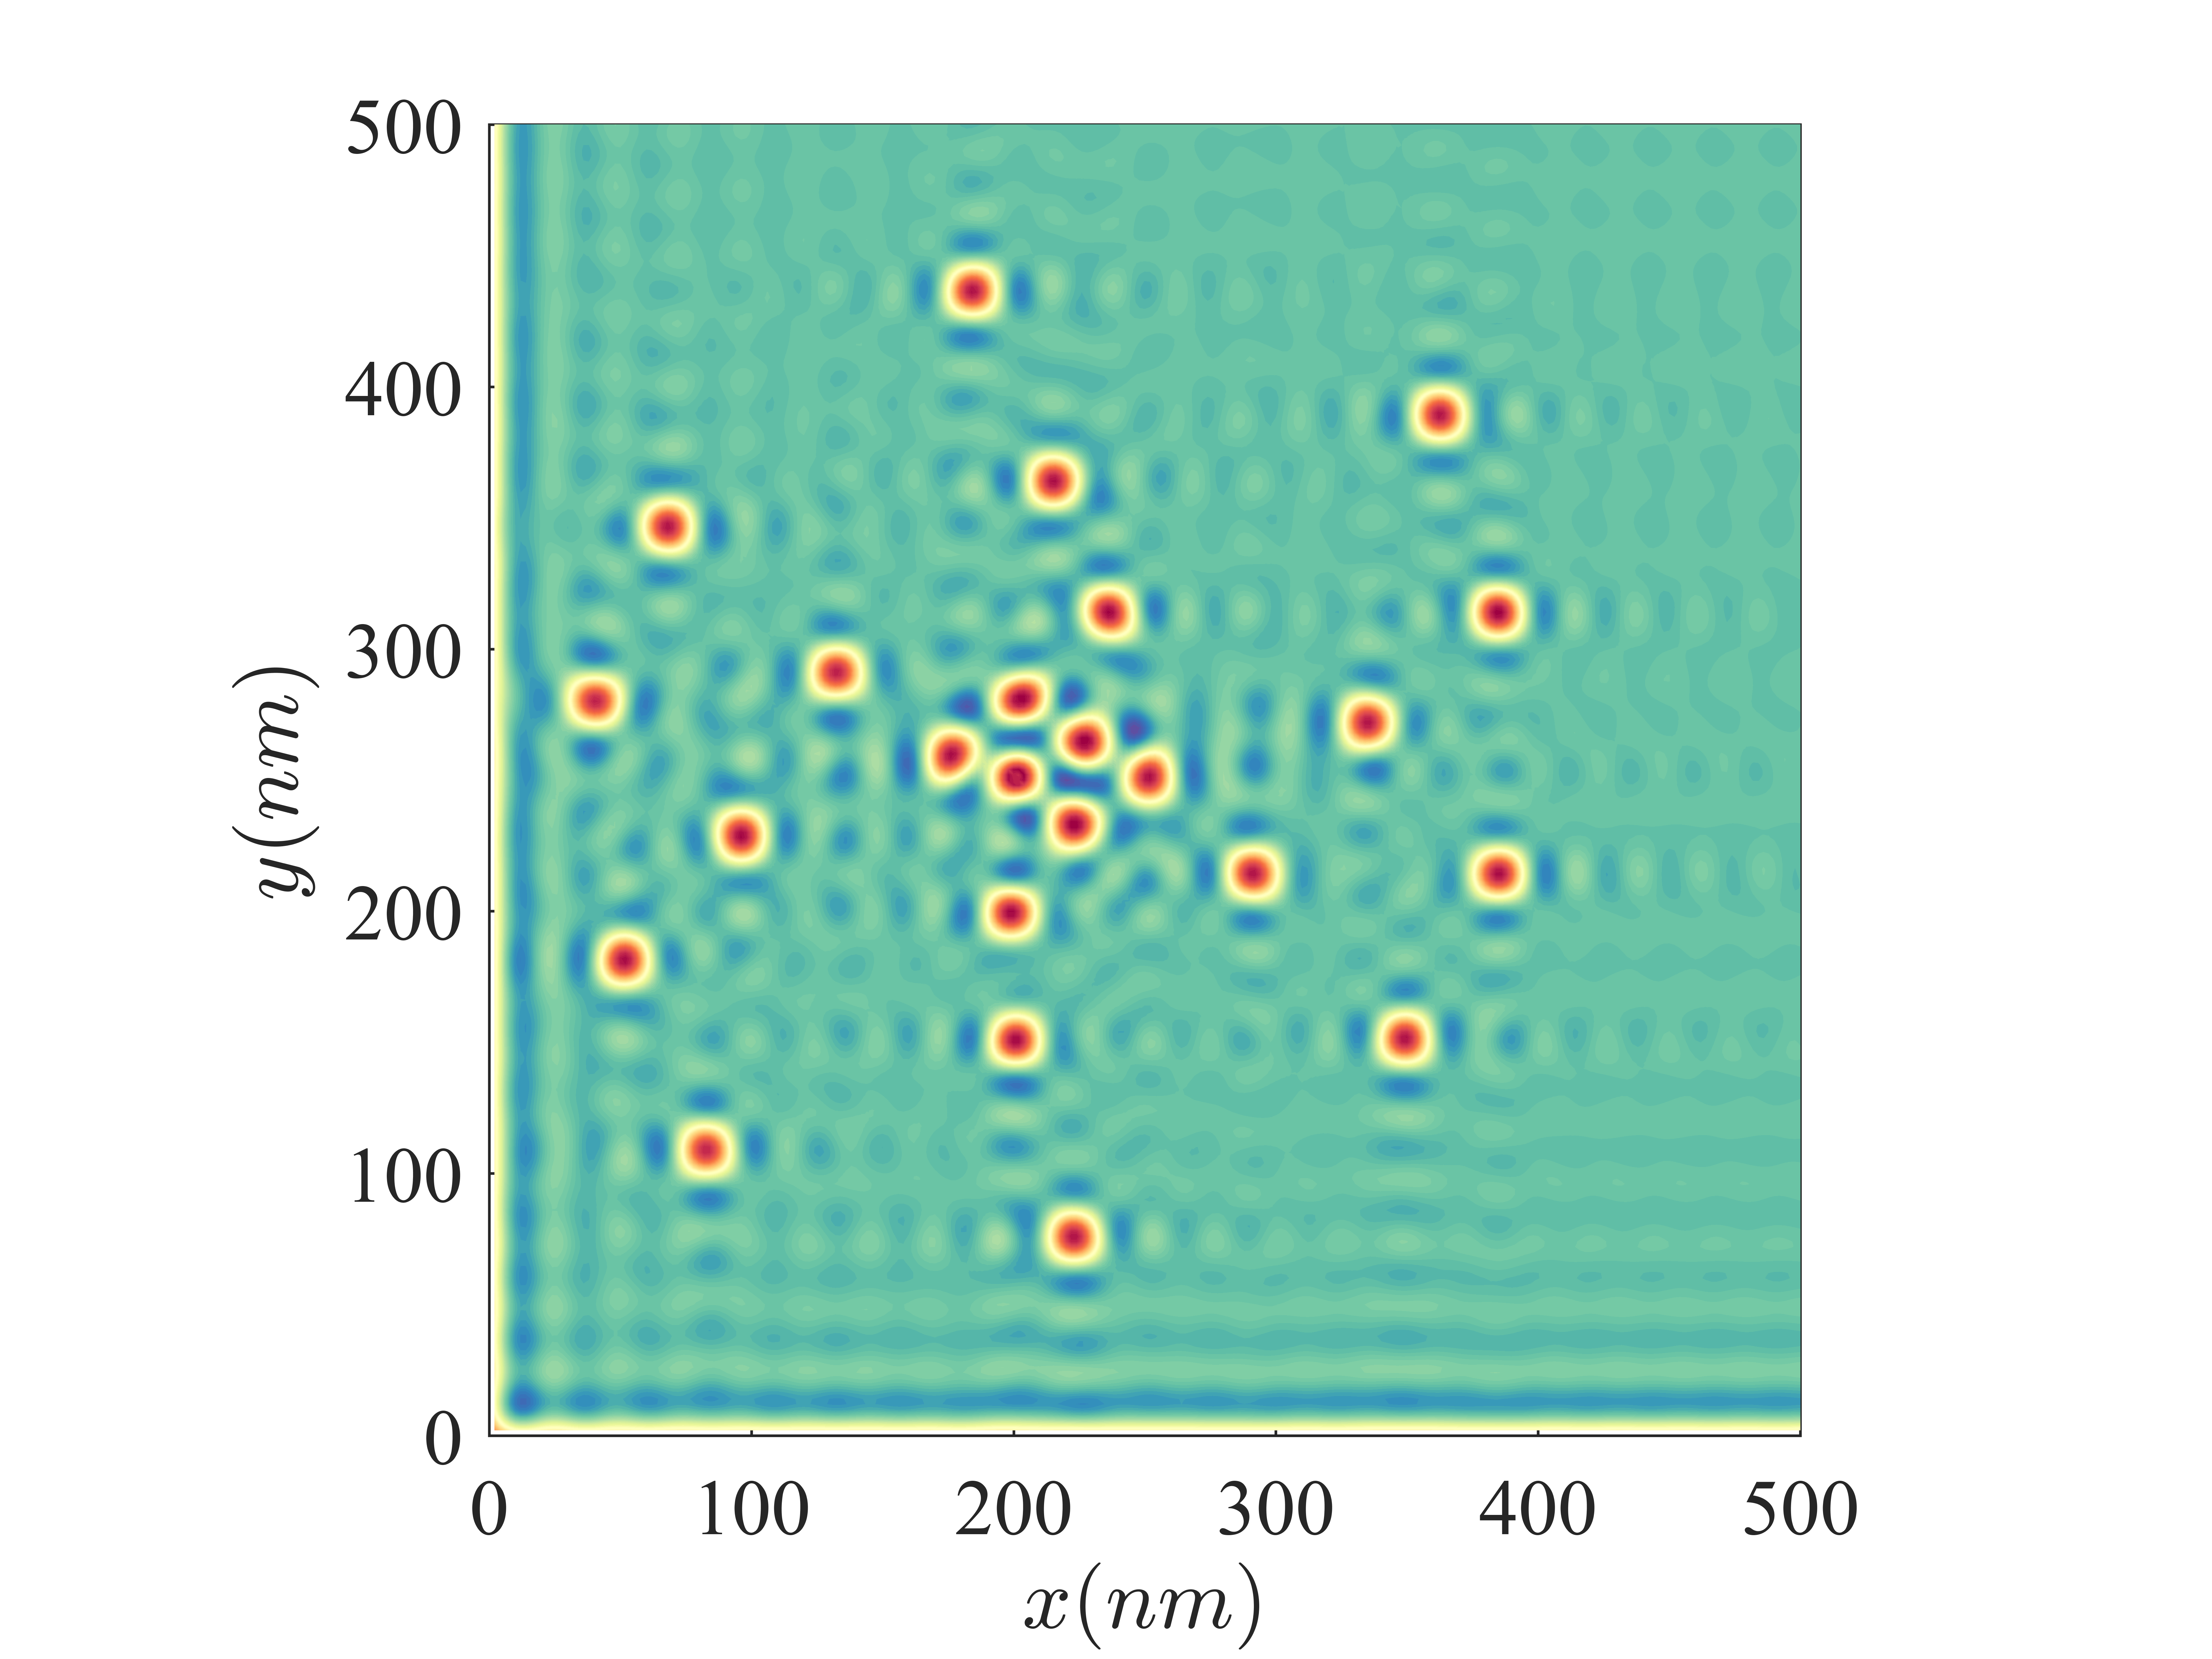
\includegraphics[scale=1]{plasmonic_sim.png}
  \caption{Simulation with GaN/AlGaN 2DEG at $25$ THz corresponding to $\Re(k_p) = 80 k_0$}
  \label{fig:plasmonic_sim}
\end{figure}

\clearpage % Force Bibliography to the end of document on a new page
\bibliography{zubairy}
\bibliographystyle{ieeetr}

\end{document}
